\section{LATAR BELAKANG}
\begin{frame}
    \frametitle{Latar Belakang}
       \vspace{-0.5cm}
  \begin{columns}
  \small
    \begin{column}{0.5\textwidth}

             \begin{figure}
             \centering
             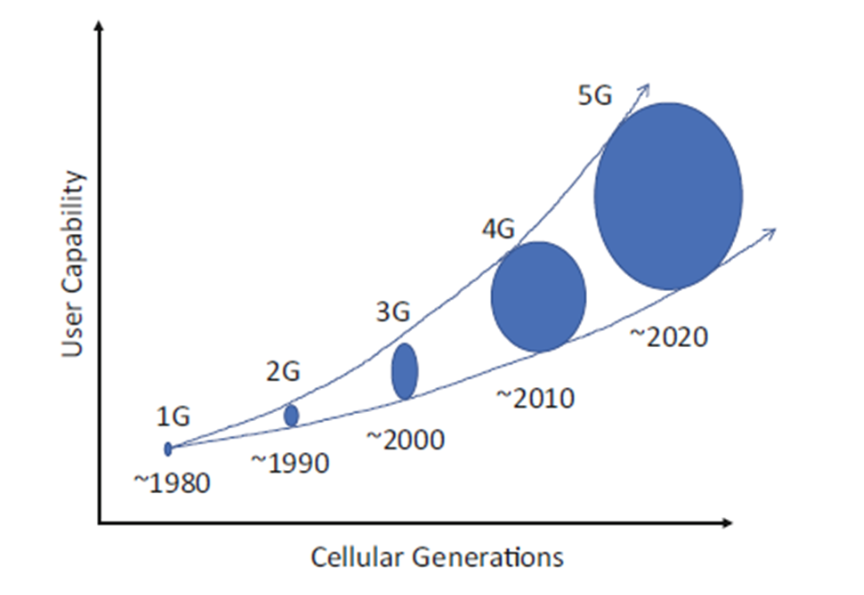
\includegraphics[width=1\textwidth]{gambar/BASIC/cellular generation.png}
             \captionsetup{font=tiny, justification=justified,width=1\textwidth}
             \captionof{figure}{Perkembangan \textit{user capability} berdasarkan \textit{cellular generations.}}
             \label{fig:cellular generation}
            \end{figure}

    \end{column}

    \begin{column}{0.5\textwidth}

\begin{itemize}\tiny \justifying   
    \item Kemampuan pengguna seluler dengan fitur yang diharapkan berkembang secara eksponensial selama evolusi generasi seluler.\\
    \item Teknologi komunikasi terus berkembang pesat, mendorong kebutuhan akan akses data yang lebih cepat dan efisien.\\
    \item Selain itu, pengguna selular terus meningkat khususnya di Indonesia selama 1 dekade mengalami peningkatan sebesar 68\% \cite{annur2022kepemilikan}.\\
    \item Seiring bertambahnya jumlah pengguna seluler, teknik akses jamak berperan dalam mengatasi keterbatasan sumber daya dan meningkatkan efisiensi pada saluran komunikasi.\\
    \item Teknik multiple access yang biasanya digunakan yaitu: TDMA (\textit{Time Division Multiple Access}), FDMA (\textit{Frequency Division Multiple Access}), CDMA (\textit{Code Division Multiple Access}), dan OFDMA (\textit{Orthogonal Frequency Division Multiple Access}).\\
    \item Dalam hal kecepatan dan efisiensi, teknologi kuantum dapat dipertimbangkan karena proses komputasinya dilakukan secara paralel.\\
    \item Pada Komputasi kuantum, kriptografi kuantum, dan komunikasi kuantum \textit{entanglement} memiliki potensi untuk menyediakan komunikasi yang sangat aman dan efisien.\\
    \item Pada penelitian ini mencoba untuk menganalisis seberapa potensial \textit{entanglement} untuk diadaptasi kedalam \textit{multiple access Channel} yang berbasis kuantum.
    
\end{itemize}
  
    \end{column}
   \end{columns}   
\end{frame}


\section{PENDAHULUAN}
\begin{frame}
\frametitle{Basic Quantum Information}
    \begin{columns}
        \begin{column}{0.5\textwidth}
            \begin{itemize}\tiny 
                \item Quantum Bit \\
                    \justifying 
                    Dalam teori quantum, terdapat unit dasar informasi yang disebut qubit. Qubit adalah sistem quantum yang memiliki dua keadaan fisik yang berbeda, yang dapat direpresentasikan sebagai \(\ket{0}\) dan \(\ket{1}\) \cite{barnett2009quantum}. Selain itu, qubit memiliki sifat superposisi yang memungkinkan untuk berada dalam keadaan superposisi dari \(\ket{0}\) dan \(ket{1}\) secara bersamaan yang dapat direpresentasikan oleh vektor dua dimensi
                        \begin{equation}
                            \ket{0} = 
                                        \begin{bmatrix}
                                            1 \\
                                            0
                                        \end{bmatrix},
                            \quad
                            \ket{1} = 
                                        \begin{bmatrix}
                                            0 \\
                                            1
                                        \end{bmatrix}.
                            \label{eq:ketket0}
                        \end{equation}
                
                \item Bloch Shapire\\
                    %\begin{columns}
                        \begin{minipage}[c]{0.3\textwidth}
                            \begin{figure}
                                \centering
                                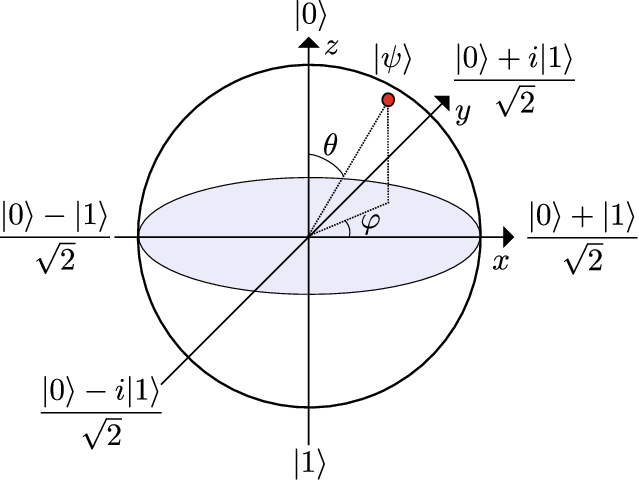
\includegraphics[width=0.9\textwidth]{gambar/BASIC/Bloch-Shapire.png}
                                \captionsetup{font=tiny} % Ukuran teks caption diset ke tiny
                                \caption{Bola Bloch}
                                \label{fig:label_gambar}
                            \end{figure}
                        \end{minipage}%
                        \begin{minipage}[c]{0.6\textwidth}
                            \tiny Bola Bloch adalah representasi geometris dari keadaan kuantum dalam mekanika kuantum yang digunakan untuk menggambarkan keadaan kuantum dari satu qubit. Setiap titik di permukaan bola Bloch mewakili satu keadaan kuantum yang mungkin dari satu qubit. Secara umum dapat dilihat melalui persamaan
                                \begin{equation}
                                    \ket{\psi} = \cos\left(\frac{\theta}{2}\right)\ket{0} + e^{i\phi}\sin\left(\frac{\theta}{2}\right)\ket{1},
                                \end{equation}   
                        \end{minipage}
                   % \end{columns}
            \end{itemize}        
        \end{column}
        
        \begin{column}{0.5\textwidth}\tiny 
\begin{equation}
\begin{aligned}
|\psi\rangle &= \alpha |0\rangle + \beta |1\rangle \\
&= \alpha
\begin{bmatrix}
1 \\
0
\end{bmatrix}
+ \beta
\begin{bmatrix}
0 \\
1
\end{bmatrix} \\
&=
\begin{bmatrix}
\alpha \\
\beta
\end{bmatrix}
\end{aligned}
\label{eq:psi}
\end{equation}

            di mana $|\alpha|^2 + |\beta|^2 = 1$ dengan \(\ket{\psi}\) adalah keadaan kuantum yang diwakili oleh titik di permukaan \textit{bola Bloch}, \(\theta\) adalah sudut polar, dan \(\phi\) adalah sudut azimut.\\
            
        \end{column}
    \end{columns}
\end{frame}
\vspace{-1cm}
\begin{frame}
  \frametitle{Quantum Entanglement}
\begin{figure}
    \centering
    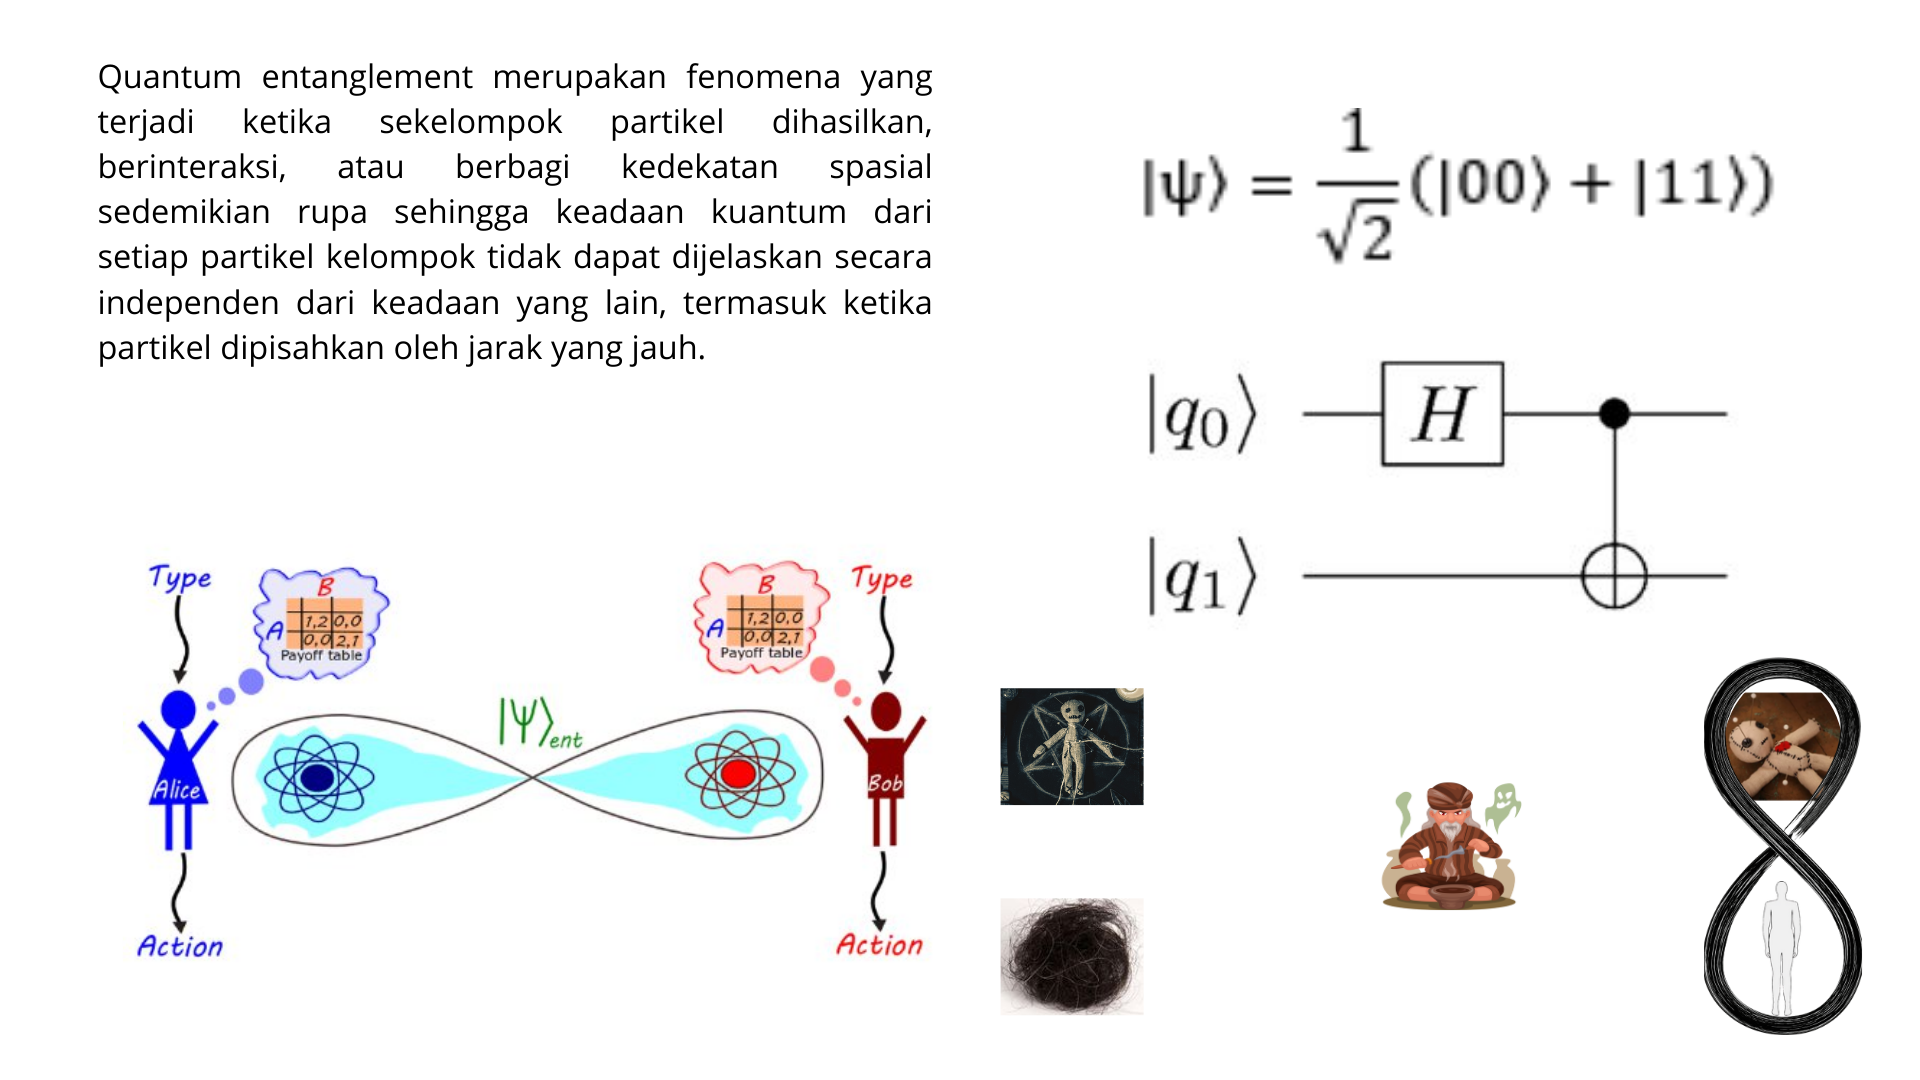
\includegraphics[width=0.8\textwidth]{gambar/BASIC/entanglement.png}
    \caption{Caption}
    \label{fig:enter-label}
\end{figure}
\end{frame}

\section{ENTROPY}
\begin{frame}
    \frametitle{Entropy 1/3}
       \vspace*{-0.5cm}
  \begin{columns}[T]
  \small
    \begin{column}{0.5\textwidth}
        \begin{itemize}
            \item Entropi \cite{djordjevic2019physical}\\
                \begin{itemize}
                \tiny \justifying                
                    \item[$\Rightarrow$] Entropi adalah ukuran dari ketidakpastian atau kekacauan dalam suatu sistem atau distribusi probabilitas.
                    \item[$\Rightarrow$]  Dalam teori informasi, entropi digunakan untuk mengukur seberapa banyak informasi yang terkandung dalam suatu variabel acak. 
                    \item[$\Rightarrow$] Entropi memiliki keterkaitan dengan konsep ketidakpastian dalam sistem, di mana semakin tinggi entropi suatu sistem, semakin tinggi pula ketidakpastian atau kekacauan dalam sistem tersebut.
                \end{itemize}
            \item Conditional Entropy\\
                \begin{itemize}
                \tiny \justifying
                    \item[$\Rightarrow$] \textit{Conditional entropy} adalah ukuran ketidakpastian yang tersisa pada input saluran setelah output saluran diterima.
                    \item[$\Rightarrow$]  \textit{Conditional entropy} mengukur seberapa banyak informasi yang masih tidak diketahui pada input saluran setelah melihat output saluran.
                    \item[$\Rightarrow$] \textit{Conditional entropy} dapat diukur melalui persamaan
                        \begin{equation}
                            H(Y|X) = -\sum_{x \in X} p(x) \sum_{y \in Y}  \, p(y|x) \log p(y|x),
                        \end{equation}
                     di mana $p(x,y)$ adalah \textit{joint distribution} dari input dan output saluran.
                \end{itemize}
        \end{itemize}
    \end{column}

   \begin{column}{0.5\textwidth}
        \begin{itemize}
            \item Relative Entropy \cite{wolfowitz2012coding}\\
                \begin{itemize}
                \tiny \justifying                
                    \item[$\Rightarrow$] Relative Entropy, juga dikenal sebagai Kullback-Leibler (KL) distance, adalah ukuran jarak antara dua distribusi probabilitas.
                    \item[$\Rightarrow$]   Relative Entropy mengukur ketidakefisiesi antara dua jarak distribusi probabilitas dengan mengasumsikan distribusi q(x) ketika distribusi sebenarnya adalah p(x). 
                    \item[$\Rightarrow$] Relative Entropy dapat diukur melalui persamaan 
                        \begin{equation}
                            D(p||q) = \sum p(x) \log\left(\frac{p(x)}{q(x)}\right).
                        \end{equation}
                \end{itemize}
            \item Mutual Information \cite{djordjevic2019physical}\\
                \begin{itemize}
                \tiny \justifying
                    \item[$\Rightarrow$] Mutual Information adalah ukuran seberapa banyak informasi yang dikandung oleh satu variabel acak terkait dengan variabel acak lainnya..
                    \item[$\Rightarrow$]  Mutual Information mengukur seberapa banyak informasi yang diketahui pada input saluran setelah melihat output saluran.
                    \item[$\Rightarrow$]Mutual Information dapat diukur melalui persamaan
                        \begin{equation}
                           I(X;Y) = H(X) - H(X|Y),
                        \end{equation}
                     di mana $H(X)$ adalah entropy dari output saluran dan $H(X|Y)$ adalah conditional entropy.
                \end{itemize}
        \end{itemize}
    \end{column}
  \end{columns}   
\end{frame}

\begin{frame}
    \frametitle{Entropy 2/3}
       \vspace*{-0.5cm}
  \begin{columns}[T]
  \small
    \begin{column}{0.5\textwidth}
        \begin{figure}
             \centering
             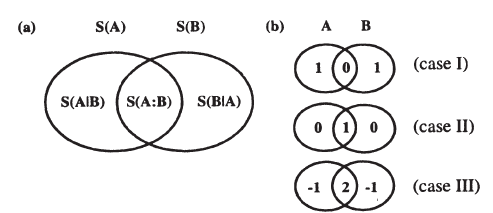
\includegraphics[width=1\textwidth]{gambar/DIAGRAM/diagram2.png}
             \captionsetup{font=tiny, justification=justified,width=1\textwidth}
             \captionof{figure}{(a) Diagram entropi umum untuk sistem komposit kuantum AB. (b) Diagram entropi untuk tiga kasus sistem 2 qubit: (I) independen, (II) terkorelasi secara klasik, (III) kuantum \textit{entanglement}.}
             \label{fig:EPR-Triplet}
        \end{figure}
        \begin{itemize} \tiny \justifying
        \vspace{-0.6 cm}
            \item Entropi von Neumann Persamaan \ref{Entropi von Neumann} diperkenalkan dalam mekanika kuantum, terkait dengan entropi Boltzmann-Gibbs-Shannon Persamaan \ref{entropi Boltzmann-Gibbs-Shannon} pada situasi klasik tertentu.
                \begin{equation}
                    S(p) = -\text{Tr}(p \log p)
                    \label{Entropi von Neumann}
                \end{equation}
                \begin{equation}
                    H(p) = -\sum_i P_i \log P_i
                    \label{entropi Boltzmann-Gibbs-Shannon}
                \end{equation}
                
        \end{itemize}
    \end{column}

   \begin{column}{0.5\textwidth}
        \begin{itemize} \tiny \justifying
            \item Density matrix  subsistem AB\\
                Ketika kita melacak derajat kebebasan yang terkait dengan C, maka matriks densitas marginal untuk subsistem AB menjadi
                    \begin{equation}
                        \rho_{AB}=\text{Tr}_c[\rho_{ABc}]=\frac{1}{2}(\ket{00}\bra{00}+\ket{11}\bra{11}),
                        \label{density matrix AB}
                    \end{equation} 
                yang sesuai dengan sistem klasik yang berkorelasi.
            \item Entropy Negative\\
                Apabila memasukkan Persamaan \ref{density matrix AB} ke dalam Persamaan \ref{Entropi von Neumann} maka menghasilkan $S(A|B)=-1$. Persamaan conditional entropy dapat dituliskan sebagai
                \begin{equation}
                    S(A|B) \equiv S(AB) - S(B).
                \end{equation}
             \item Fungsi Negative Conditional Entropy\\
                Dalam konteks sistem kuantum komposit yang tidak diketahui, konsep entropi kondisional negatif terbukti sangat berguna dalam menjelaskan sistem kuantum yang terdiri dari beberapa bagian, serta memberikan pemahaman baru tentang pembentukan korelasi klasikal dari \textit{quantum entanglement}.
        \end{itemize}
    \end{column}
  \end{columns}   
\end{frame}

\begin{frame}
    \frametitle{Entropy 3/3}
       \vspace*{-0.5cm}
  \begin{columns}[T]
  \tiny
    \begin{column}{0.5\textwidth}
\begin{align*}
\ket{\psi_{AB}} &= \frac{1}{2} (\ket{00} + \ket{11}){AB}. \\
\rho_{AB} &= \ket{\psi_{AB}}\bra{\psi_{AB}} \\
&= \frac{1}{2} (\ket{00} + \ket{11})_{AB} \otimes (\bra{00} + \bra{11}){AB}.\\
&= \frac{1}{2}(\ket{00}\bra{00}+\ket{00}\bra{11}+\ket{11}\bra{00}+\ket{11}\bra{11})\\
\hat{\rho}_A &= \text{tr}B (\rho{AB})\\
&= \frac{1}{2} \left( |0\rangle\langle 0|_A \text{tr} (|0\rangle\langle 0|_B) + |0\rangle\langle 1|_A \text{tr} (|0\rangle\langle 1|_B) \right. \\
& \quad + \left. |1\rangle\langle 0|_A \text{tr} (|1\rangle\langle 0|_B) + |1\rangle\langle 1|_A \text{tr} (|1\rangle\langle 1|_B) \right) \\
&= \frac{1}{2} (|0\rangle\langle 0|_A + |1\rangle\langle 1|_A) \\
&\equiv \frac{1}{2} I_A \\
\end{align*}
    \end{column}

   \begin{column}{0.5\textwidth}
   
\begin{align*}
\hat{\rho}_B &= \text{tr}_A(\rho_{AB}) \\
&= \frac{1}{2} \left[ \text{tr}(|0\rangle\langle 0|_A) \cdot |0\rangle\langle 0|_B + \text{tr}(|0\rangle\langle 1|_A) \cdot |0\rangle\langle 1|_B \right. \\
& \quad + \left. \text{tr}(|1\rangle\langle 0|_A) \cdot |1\rangle\langle 0|_B + \text{tr}(|1\rangle\langle 1|_A) \cdot |1\rangle\langle 1|_B \right] \\
&= \frac{1}{2} (|0\rangle\langle 0|_B + |1\rangle\langle 1|_B) \\
&\equiv \frac{1}{2} I_B.\\
\hat{\rho}_A \otimes \hat{\rho}_B &= I_A \frac{1}{2} \otimes I_B \frac{1}{2} \\
&= I_{AB} \frac{1}{4} \\
&\equiv \frac{1}{4} (|00\rangle\langle00| + |01\rangle\langle01| + |10\rangle\langle10| + |11\rangle\langle11|).\\
S(\hat{\rho}_A) &= S(\hat{\rho}_B) = -2 \times \left(\frac{1}{2}\right) \log\left(\frac{1}{2}\right) \equiv 1.\\
S(\rho_A | \rho_B) &= S(\rho_{AB}) - S(\hat{\rho}_B) = 0 - 1 \equiv -1 \\
S(\rho_B | \rho_A) &= S(\rho_{AB}) - S(\hat{\rho}_A) = 0 - 1 \equiv -1.
\end{align*}

    \end{column}
  \end{columns}  
\end{frame}
\begin{frame}
    \frametitle{Slepian–Wolf Bound}
       \vspace{-0.5cm}
  \begin{columns}
  \small
    \begin{column}{0.5\textwidth}
        \begin{itemize} 
             \begin{figure}
             \centering
             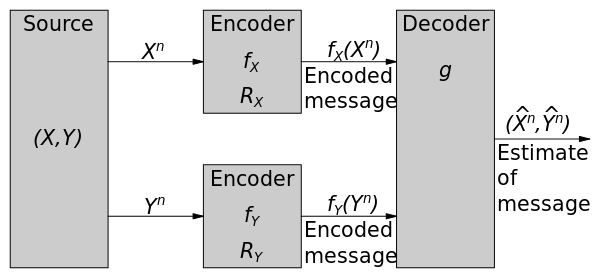
\includegraphics[width=0.8\textwidth]{gambar/BASIC/SlepianWolfEncoderDecoder.png}
             \captionsetup{font=tiny, justification=justified,width=1\textwidth}
             \captionof{figure}{Dua sumber distribusi random X dan Y yang melalui encoder decoder.}
             \label{fig:encoderdecoderslepianwolf}
            \end{figure}
    \justifying \tiny \vspace{-0.5cm}
            \item Slepian–Wolf bound adalah batasan entropi yang menentukan jumlah bit minimum yang dibutuhkan untuk mengkodekan dua sumber data yang berkorelasi secara lossless yang ditemukan oleh David Slepian dan Jack Wolf pada tahun 1973.
            \item Batasan ini menyatakan bahwa untuk mengkodekan dua sumber data yang berkorelasi secara lossless, laju bit total harus setidaknya sama dengan jumlah entropi sumber individu dikurangi informasi bersama.
            \item Jika dua sumber data berkorelasi secara kuat, maka informasi yang diperlukan untuk mengkodekan satu sumber data dapat dikurangi dengan menggunakan informasi dari sumber data lainnya. 
    
        \end{itemize}
    \end{column}

    \begin{column}{0.5\textwidth}

       \tiny \justifying
             \begin{figure}
             \centering
             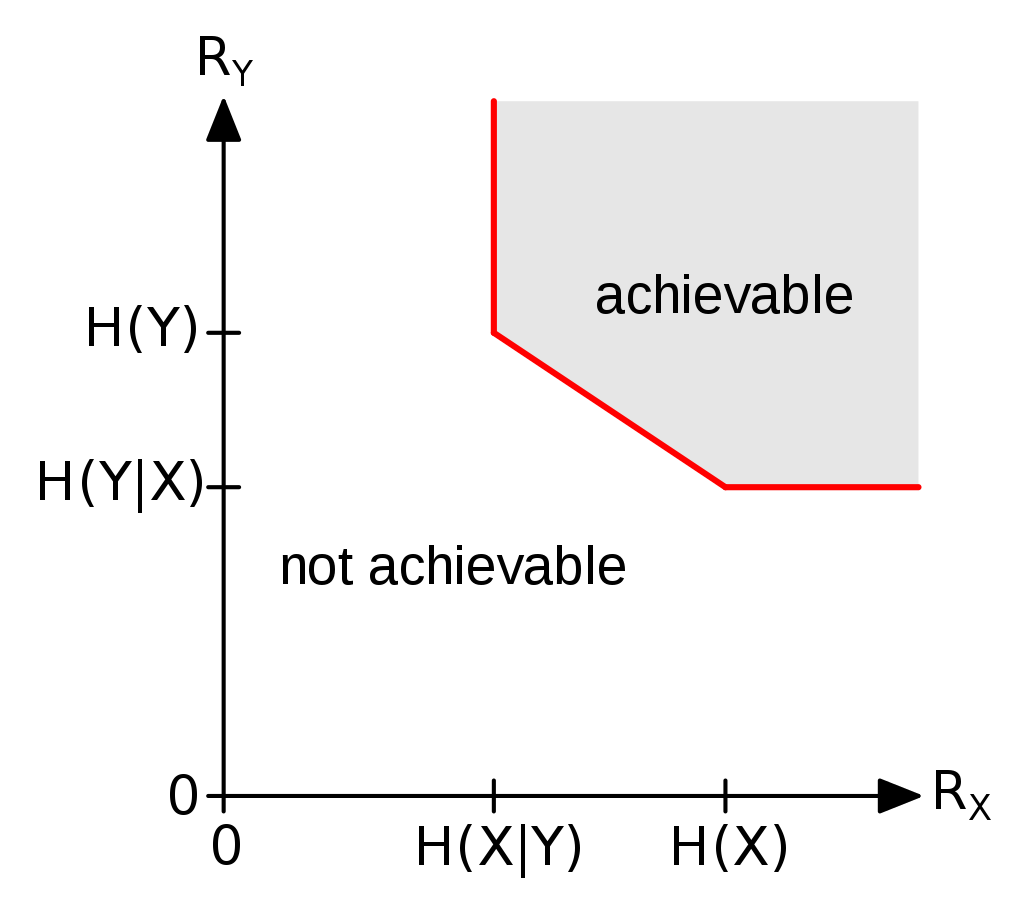
\includegraphics[width=0.5\textwidth]{gambar/BASIC/SlepianWolfPlot.png}
             \captionsetup{font=tiny, justification=justified,width=1\textwidth}
             \captionof{figure}{Batas tingkat lossless coding pada dua sumber X dan Y.}
             \label{fig:encoderdecoderslepianwolf}
            \end{figure} \vspace{-0.8cm}
                \begin{align*}
                    R_X &\geq H(X|Y) \\
                    R_Y &\geq H(Y|X) \\
                    R_X + R_Y &\geq H(X,Y)
                \end{align*}
        Sumber catatan \firstcite{slepian1973noiseless}
  
    \end{column}
   \end{columns}   
\end{frame}

\section{KESIMPULAN}
\begin{frame}{KESIMPULAN}
    \begin{itemize}\justifying
        \item Analisis \textit{multiple access on quantum entanglement} bertujuan untuk mengeksplorasi bagaimana entanglement kuantum dapat dimanfaatkan untuk meningkatkan efisiensi dan keamanan pada jaringan komunikasi.
        \item  Entropi kondisional negatif berfungsi untuk menje-
laskan sistem kuantum yang terdiri dari beberapa bagian, serta mem-
berikan pemahaman baru tentang pembentukan korelasi klasikal dari
quantum entanglement.
    \end{itemize}
\end{frame}
